\columnratio{0.55}
\begin{paracol}{2}
\switchcolumn[0]*%%%%%%%
\section{Components Basics}
\switchcolumn
\section{组件基础}
\switchcolumn[0]*%%%%%%%
Components allow us to split the UI into independent and reusable
pieces, and think about each piece in isolation. It's common for an app
to be organized into a tree of nested components:
\switchcolumn
组件允许我们将 UI
划分为独立的、可重用的部分,并且可以对每个部分进行单独的思考。在实际应用中,组件常常被组织成层层嵌套的树状结构:
\end{paracol}


\begin{center} 
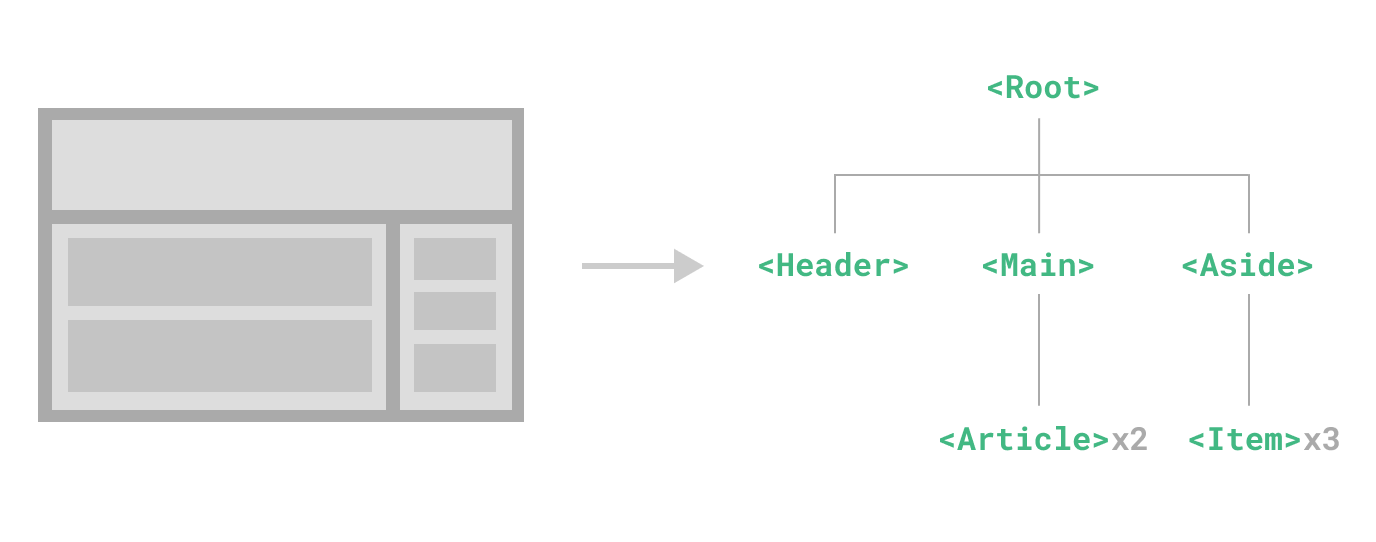
\includegraphics{./img/components.7fbb3771.png} 
\end{center}

\columnratio{0.55}
\begin{paracol}{2}

\switchcolumn[0]*%%%%%%%
This is very similar to how we nest native HTML elements, but Vue
implements its own component model that allow us to encapsulate custom
content and logic in each component. Vue also plays nicely with native
Web Components. If you are curious about the relationship between Vue
Components and native Web Components,
\href{https://vuejs.org/guide/extras/web-components.html}{read more
here}.
\switchcolumn
这和我们嵌套 HTML 元素的方式类似,Vue
实现了自己的组件模型,使我们可以在每个组件内封装自定义内容与逻辑。Vue
同样也能很好地配合原生 Web Component。如果你想知道 Vue 组件与原生 Web
Components
之间的关系,可以\href{https://cn.vuejs.org/guide/extras/web-components.html}{阅读此章节}。
\switchcolumn[0]*%%%%%%%
\subsection{Defining a Component}
\switchcolumn
\subsection{定义一个组件}
\switchcolumn[0]*%%%%%%%
When using a build step, we typically define each Vue component in a
dedicated file using the \texttt{.vue} extension - known as a
\href{https://vuejs.org/guide/scaling-up/sfc.html}{Single-File
Component} (SFC for short):
\switchcolumn
当使用构建步骤时,我们一般会将 Vue 组件定义在一个单独的 \texttt{.vue}
文件中,这被叫做\href{https://cn.vuejs.org/guide/scaling-up/sfc.html}{单文件组件}
(简称 SFC):
\switchcolumn[0]*%%%%%%%
\begin{codeHtml}
<script setup>
import { ref } from 'vue'
//
const count = ref(0)
</script>
//
<template>
    <button @click="count++">You clicked me {{ count }} times.</button>
</template>
\end{codeHtml}
\switchcolumn
\begin{codeHtml}
<script setup>
import { ref } from 'vue'
//
const count = ref(0)
</script>
//
<template>
    <button @click="count++">You clicked me {{ count }} times.</button>
</template>
\end{codeHtml}
\switchcolumn[0]*%%%%%%%
When not using a build step, a Vue component can be defined as a plain
JavaScript object containing Vue-specific options:
\switchcolumn
当不使用构建步骤时,一个 Vue 组件以一个包含 Vue 特定选项的 JavaScript
对象来定义:


\switchcolumn[0]*%%%%%%%
\begin{codeJs}
import { ref } from 'vue'
//
export default {
  setup() {
    const count = ref(0)
    return { count }
  },
  template: `
    <button @click="count++">
      You clicked me {{ count }} times.
    </button>`
  // 也可以针对一个 DOM 内联模板:
  // template: '#my-template-element'
}
\end{codeJs}
\switchcolumn
\begin{codeJs}
import { ref } from 'vue'
//
export default {
  setup() {
    const count = ref(0)
    return { count }
  },
  template: `
    <button @click="count++">
      You clicked me {{ count }} times.
    </button>`
  // 也可以针对一个 DOM 内联模板:
  // template: '#my-template-element'
}
\end{codeJs}
\switchcolumn[0]*%%%%%%%
The template is inlined as a JavaScript string here, which Vue will
compile on the fly. You can also use an ID selector pointing to an
element (usually native \texttt{\textless{}template\textgreater{}}
elements) - Vue will use its content as the template source.
\switchcolumn
这里的模板是一个内联的 JavaScript 字符串,Vue
将会在运行时编译它。你也可以使用 ID 选择器来指向一个元素 (通常是原生的
\texttt{\textless{}template\textgreater{}} 元素),Vue
将会使用其内容作为模板来源。
\switchcolumn[0]*%%%%%%%
The example above defines a single component and exports it as the
default export of a \texttt{.js} file, but you can use named exports to
export multiple components from the same file.
\switchcolumn
上面的例子中定义了一个组件,并在一个 \texttt{.js}
文件里默认导出了它自己,但你也可以通过具名导出在一个文件中导出多个组件。
\switchcolumn[0]*%%%%%%%
\subsection{Using a Component}
\switchcolumn
\subsection{使用组件}
\switchcolumn[0]*%%%%%%%
\begin{vueQuote}{TIP}
We will be using SFC syntax for the rest of this guide - the concepts
around components are the same regardless of whether you are using a
build step or not. The \href{https://vuejs.org/examples/}{Examples}
section shows component usage in both scenarios.
\end{vueQuote}
\switchcolumn
\begin{vueQuote}{TIP}
我们会在接下来的指引中使用 SFC
语法,无论你是否使用构建步骤,组件相关的概念都是相同的。\href{https://cn.vuejs.org/examples/}{示例}一节中展示了两种场景中的组件使用情况。
\end{vueQuote}


\switchcolumn[0]*%%%%%%%
To use a child component, we need to import it in the parent component.
Assuming we placed our counter component inside a file called
\texttt{ButtonCounter.vue}, the component will be exposed as the file's
default export:
\switchcolumn
要使用一个子组件,我们需要在父组件中导入它。假设我们把计数器组件放在了一个叫做
\texttt{ButtonCounter.vue}
的文件中,这个组件将会以默认导出的形式被暴露给外部。
\switchcolumn[0]*%%%%%%%
\begin{codeHtml}
<script setup>
import ButtonCounter from './ButtonCounter.vue'
</script>
<!-- -->
<template>
  <h1>Here is a child component!</h1>
  <ButtonCounter />
</template>
\end{codeHtml}
\switchcolumn
\begin{codeHtml}
<script setup>
import ButtonCounter from './ButtonCounter.vue'
</script>
<!-- -->
<template>
  <h1>Here is a child component!</h1>
  <ButtonCounter />
</template>
\end{codeHtml}
\switchcolumn[0]*%%%%%%%
With \texttt{\textless{}script\ setup\textgreater{}}, imported
components are automatically made available to the template.
\switchcolumn
通过
\texttt{\textless{}script\ setup\textgreater{}},导入的组件都在模板中直接可用。
\switchcolumn[0]*%%%%%%%
It's also possible to globally register a component, making it available
to all components in a given app without having to import it. The pros
and cons of global vs. local registration is discussed in the dedicated
\href{https://vuejs.org/guide/components/registration.html}{Component
Registration} section.
\switchcolumn
当然,你也可以全局地注册一个组件,使得它在当前应用中的任何组件上都可以使用,而不需要额外再导入。关于组件的全局注册和局部注册两种方式的利弊,我们放在了\href{https://cn.vuejs.org/guide/components/registration.html}{组件注册}这一章节中专门讨论。
\switchcolumn[0]*%%%%%%%
Components can be reused as many times as you want:
\switchcolumn
组件可以被重用任意多次:


\switchcolumn[0]*%%%%%%%
\begin{codeHtml}
<h1>Here is a child component!</h1>
<ButtonCounter />
<ButtonCounter />
<ButtonCounter />
\end{codeHtml}
\switchcolumn
\begin{codeHtml}
<h1>Here is a child component!</h1>
<ButtonCounter />
<ButtonCounter />
<ButtonCounter />
\end{codeHtml}
\switchcolumn[0]*%%%%%%%
\href{https://play.vuejs.org/\#eNqVj91KAzEQhV/lmJsqlY3eSlr8ufEVhNys6ZQGNz8kE0GWfXez2SJUsdCLuZiZM9+ZM4qnGLvPQuJBqGySjYxMXOJWe+tiSIznwhz8SyieKWGfgsOqkyfTGbDSXsmFUG9rw+Ti0DPNHavD/faVEqGv5Xr/BXOwww4mVBNPnvOVklXTtKeO8qKhkj++4lb8+fL/mCMS7TEdAy6BtDfBZ65fVgA2s+L67uZMUEC9N0s8msGaj40W7Xa91qKtgbdQ0Ha0gyOM45E+TWDrKHeNIhfMr0DTN4U0me8=}{Try
it in the Playground}
\switchcolumn
\href{https://play.vuejs.org/\#eNqVj91KAzEQhV/lmJsqlY3eSlr8ufEVhNys6ZQGNz8kE0GWfXez2SJUsdCLuZiZM9+ZM4qnGLvPQuJBqGySjYxMXOJWe+tiSIznwhz8SyieKWGfgsOqkyfTGbDSXsmFUG9rw+Ti0DPNHavD/faVEqGv5Xr/BXOwww4mVBNPnvOVklXTtKeO8qKhkj++4lb8+fL/mCMS7TEdAy6BtDfBZ65fVgA2s+L67uZMUEC9N0s8msGaj40W7Xa91qKtgbdQ0Ha0gyOM45E+TWDrKHeNIhfMr0DTN4U0me8=}{在演练场中尝试一下}
\switchcolumn[0]*%%%%%%%
Notice that when clicking on the buttons, each one maintains its own,
separate \texttt{count}. That's because each time you use a component, a
new \textbf{instance} of it is created.
\switchcolumn
你会注意到,每当点击这些按钮时,每一个组件都维护着自己的状态,是不同的
\texttt{count}。这是因为每当你使用一个组件,就创建了一个新的\textbf{实例}。
\switchcolumn[0]*%%%%%%%
In SFCs, it's recommended to use \texttt{PascalCase} tag names for child
components to differentiate from native HTML elements. Although native
HTML tag names are case-insensitive, Vue SFC is a compiled format so we
are able to use case-sensitive tag names in it. We are also able to use
\texttt{/\textgreater{}} to close a tag.
\switchcolumn
在单文件组件中,推荐为子组件使用 \texttt{PascalCase}
的标签名,以此来和原生的 HTML 元素作区分。虽然原生 HTML
标签名是不区分大小写的,但 Vue
单文件组件是可以在编译中区分大小写的。我们也可以使用
\texttt{/\textgreater{}} 来关闭一个标签。
\switchcolumn[0]*%%%%%%%
If you are authoring your templates directly in a DOM (e.g. as the
content of a native \texttt{\textless{}template\textgreater{}} element),
the template will be subject to the browser's native HTML parsing
behavior. In such cases, you will need to use \texttt{kebab-case} and
explicit closing tags for components:
\switchcolumn
如果你是直接在 DOM 中书写模板 (例如原生
\texttt{\textless{}template\textgreater{}}
元素的内容),模板的编译需要遵从浏览器中 HTML
的解析行为。在这种情况下,你应该需要使用 \texttt{kebab-case}
形式并显式地关闭这些组件的标签。


\switchcolumn[0]*%%%%%%%
\begin{codeHtml}
<!-- 如果是在 DOM 中书写该模板 -->
<button-counter></button-counter>
<button-counter></button-counter>
<button-counter></button-counter>
\end{codeHtml}
\switchcolumn
\begin{codeHtml}
<!-- 如果是在 DOM 中书写该模板 -->
<button-counter></button-counter>
<button-counter></button-counter>
<button-counter></button-counter>
\end{codeHtml}
\switchcolumn[0]*%%%%%%%
See
\href{https://vuejs.org/guide/essentials/component-basics.html\#in-dom-template-parsing-caveats}{in-DOM
template parsing caveats} for more details.
\switchcolumn
请看
\href{https://cn.vuejs.org/guide/essentials/component-basics.html\#in-dom-template-parsing-caveats}{DOM
内模板解析注意事项}了解更多细节。
\switchcolumn[0]*%%%%%%%
\subsection{Passing Props}
\switchcolumn
\subsection{传递 props}
\switchcolumn[0]*%%%%%%%
If we are building a blog, we will likely need a component representing
a blog post. We want all the blog posts to share the same visual layout,
but with different content. Such a component won't be useful unless you
can pass data to it, such as the title and content of the specific post
we want to display. That's where props come in.
\switchcolumn
如果我们正在构建一个博客,我们可能需要一个表示博客文章的组件。我们希望所有的博客文章分享相同的视觉布局,但有不同的内容。要实现这样的效果自然必须向组件中传递数据,例如每篇文章标题和内容,这就会使用到
props。
\switchcolumn[0]*%%%%%%%
Props are custom attributes you can register on a component. To pass a
title to our blog post component, we must declare it in the list of
props this component accepts, using the
\href{https://vuejs.org/api/sfc-script-setup.html\#defineprops-defineemits}{\texttt{defineProps}}
macro:
\switchcolumn
Props 是一种特别的
attributes,你可以在组件上声明注册。要传递给博客文章组件一个标题,我们必须在组件的
props 列表上声明它。这里要用到
\href{https://cn.vuejs.org/api/sfc-script-setup.html\#defineprops-defineemits}{\texttt{defineProps}}
宏:


\switchcolumn[0]*%%%%%%%
\begin{codeHtml}
<!-- BlogPost.vue -->
<script setup>
defineProps(['title'])
</script>
<!-- -->
<template>
  <h4>{{ title }}</h4>
</template>
\end{codeHtml}
\switchcolumn
\begin{codeHtml}
<!-- BlogPost.vue -->
<script setup>
defineProps(['title'])
</script>
<!-- -->
<template>
  <h4>{{ title }}</h4>
</template>
\end{codeHtml}
\switchcolumn[0]*%%%%%%%
\texttt{defineProps} is a compile-time macro that is only available
inside \texttt{\textless{}script\ setup\textgreater{}} and does not need
to be explicitly imported. Declared props are automatically exposed to
the template. \texttt{defineProps} also returns an object that contains
all the props passed to the component, so that we can access them in
JavaScript if needed:
\switchcolumn
\texttt{defineProps} 是一个仅
\texttt{\textless{}script\ setup\textgreater{}}
中可用的编译宏命令,并不需要显式地导入。声明的 props
会自动暴露给模板。\texttt{defineProps}
会返回一个对象,其中包含了可以传递给组件的所有 props:
\switchcolumn[0]*%%%%%%%
\begin{codeJs}
const props = defineProps(['title'])
console.log(props.title)
\end{codeJs}
\switchcolumn
\begin{codeJs}
const props = defineProps(['title'])
console.log(props.title)
\end{codeJs}
\switchcolumn[0]*%%%%%%%
See also:
\href{https://vuejs.org/guide/typescript/composition-api.html\#typing-component-props}{Typing
Component Props}
\switchcolumn
TypeScript
用户请参考:\href{https://cn.vuejs.org/guide/typescript/composition-api.html\#typing-component-props}{为组件
props 标注类型}
\switchcolumn[0]*%%%%%%%
If you are not using \texttt{\textless{}script\ setup\textgreater{}},
props should be declared using the \texttt{props} option, and the props
object will be passed to \texttt{setup()} as the first argument:
\switchcolumn
如果你没有使用 \texttt{\textless{}script\ setup\textgreater{}},props
必须以 \texttt{props} 选项的方式声明,props 对象会作为 \texttt{setup()}
函数的第一个参数被传入:


\switchcolumn[0]*%%%%%%%
\begin{codeJs}
export default {
  props: ['title'],
  setup(props) {
    console.log(props.title)
  }
}
\end{codeJs}
\switchcolumn
\begin{codeJs}
export default {
  props: ['title'],
  setup(props) {
    console.log(props.title)
  }
}
\end{codeJs}
\switchcolumn[0]*%%%%%%%
A component can have as many props as you like and, by default, any
value can be passed to any prop.
\switchcolumn
一个组件可以有任意多的 props,默认情况下,所有 prop 都接受任意类型的值。
\switchcolumn[0]*%%%%%%%
Once a prop is registered, you can pass data to it as a custom
attribute, like this:
\switchcolumn
当一个 prop 被注册后,可以像这样以自定义 attribute 的形式传递数据给它:
\switchcolumn[0]*%%%%%%%
\begin{codeHtml}
<BlogPost title="My journey with Vue" />
<BlogPost title="Blogging with Vue" />
<BlogPost title="Why Vue is so fun" />
\end{codeHtml}
\switchcolumn
\begin{codeHtml}
<BlogPost title="My journey with Vue" />
<BlogPost title="Blogging with Vue" />
<BlogPost title="Why Vue is so fun" />
\end{codeHtml}
\switchcolumn[0]*%%%%%%%
In a typical app, however, you'll likely have an array of posts in your
parent component:
\switchcolumn
在实际应用中,我们可能在父组件中会有如下的一个博客文章数组:


\switchcolumn[0]*%%%%%%%
\begin{codeJs}
const posts = ref([
  { id: 1, title: 'My journey with Vue' },
  { id: 2, title: 'Blogging with Vue' },
  { id: 3, title: 'Why Vue is so fun' }
])
\end{codeJs}
\switchcolumn
\begin{codeJs}
const posts = ref([
  { id: 1, title: 'My journey with Vue' },
  { id: 2, title: 'Blogging with Vue' },
  { id: 3, title: 'Why Vue is so fun' }
])
\end{codeJs}
\switchcolumn[0]*%%%%%%%
Then want to render a component for each one, using \texttt{v-for}:
\switchcolumn
这种情况下,我们可以使用 \texttt{v-for} 来渲染它们:
\switchcolumn[0]*%%%%%%%
\begin{codeHtml}
<BlogPost
  v-for="post in posts"
  :key="post.id"
  :title="post.title"
 />
\end{codeHtml}
\switchcolumn
\begin{codeHtml}
<BlogPost
  v-for="post in posts"
  :key="post.id"
  :title="post.title"
 />
\end{codeHtml}
\switchcolumn[0]*%%%%%%%
\href{https://play.vuejs.org/\#eNp9kU9PhDAUxL/KpBfWBCH+OZEuid5N9qSHrQezFKhC27RlDSF8d1tYQBP1+N78OpN5HciD1sm54yQj1J6M0A6Wu07nTIpWK+MwwPASI0qjWkQejVbpsVHVQVl30ZJ0WQRHjwFMnpT0gPZLi32w2h2DMEAUGW5iOOEaniF66vGuOiN5j0/hajx7B4zxxt5ubIiphKz+IO828qXugw5hYRXKTnqSydcrJmk61/VF/eB4q5s3x8Pk6FJjauDO16Uye0ZCBwg5d2EkkED2wfuLlogibMOTbMpf9tMwP8jpeiMfRdM1l8Tk+/F++Y6Cl0Lyg1Ha7o7R5Bn9WwSg9X0+DPMxMI409fPP1PELlVmwdQ==}{Try
it in the Playground}
\switchcolumn
\href{https://play.vuejs.org/\#eNp9kU9PhDAUxL/KpBfWBCH+OZEuid5N9qSHrQezFKhC27RlDSF8d1tYQBP1+N78OpN5HciD1sm54yQj1J6M0A6Wu07nTIpWK+MwwPASI0qjWkQejVbpsVHVQVl30ZJ0WQRHjwFMnpT0gPZLi32w2h2DMEAUGW5iOOEaniF66vGuOiN5j0/hajx7B4zxxt5ubIiphKz+IO828qXugw5hYRXKTnqSydcrJmk61/VF/eB4q5s3x8Pk6FJjauDO16Uye0ZCBwg5d2EkkED2wfuLlogibMOTbMpf9tMwP8jpeiMfRdM1l8Tk+/F++Y6Cl0Lyg1Ha7o7R5Bn9WwSg9X0+DPMxMI409fPP1PELlVmwdQ==}{在演练场中尝试一下}
\switchcolumn[0]*%%%%%%%
Notice how \texttt{v-bind} is used to pass dynamic prop values. This is
especially useful when you don't know the exact content you're going to
render ahead of time.
\switchcolumn
留意我们是如何使用 \texttt{v-bind} 来传递动态 prop
值的。当事先不知道要渲染的确切内容时,这一点特别有用。


\switchcolumn[0]*%%%%%%%
That's all you need to know about props for now, but once you've
finished reading this page and feel comfortable with its content, we
recommend coming back later to read the full guide on
\href{https://vuejs.org/guide/components/props.html}{Props}.
\switchcolumn
以上就是目前你需要了解的关于 props
的全部了。如果你看完本章节后还想知道更多细节,我们推荐你深入阅读关于
props
的\href{https://cn.vuejs.org/guide/components/props.html}{完整指引}。
\switchcolumn[0]*%%%%%%%
\subsection{Listening to Events}
\switchcolumn
\subsection{监听事件}
\switchcolumn[0]*%%%%%%%
As we develop our \texttt{\textless{}BlogPost\textgreater{}} component,
some features may require communicating back up to the parent. For
example, we may decide to include an accessibility feature to enlarge
the text of blog posts, while leaving the rest of the page at its
default size.
\switchcolumn
让我们继续关注我们的 \texttt{\textless{}BlogPost\textgreater{}}
组件。我们会发现有时候它需要与父组件进行交互。例如,要在此处实现无障碍访问的需求,将博客文章的文字能够放大,而页面的其余部分仍使用默认字号。
\switchcolumn[0]*%%%%%%%
In the parent, we can support this feature by adding a
\texttt{postFontSize} ref:
\switchcolumn
在父组件中,我们可以添加一个 \texttt{postFontSize} ref 来实现这个效果:
\switchcolumn[0]*%%%%%%%
\begin{codeJs}
const posts = ref([
  /* ... */
])
//
const postFontSize = ref(1)
\end{codeJs}
\switchcolumn
\begin{codeJs}
const posts = ref([
  /* ... */
])
//
const postFontSize = ref(1)
\end{codeJs}


\switchcolumn[0]*%%%%%%%
Which can be used in the template to control the font size of all blog
posts:
\switchcolumn
在模板中用它来控制所有博客文章的字体大小:
\switchcolumn[0]*%%%%%%%
\begin{codeHtml}
<div :style="{ fontSize: postFontSize + 'em' }">
  <BlogPost
    v-for="post in posts"
    :key="post.id"
    :title="post.title"
   />
</div>
\end{codeHtml}
\switchcolumn
\begin{codeHtml}
<div :style="{ fontSize: postFontSize + 'em' }">
  <BlogPost
    v-for="post in posts"
    :key="post.id"
    :title="post.title"
   />
</div>
\end{codeHtml}
\switchcolumn[0]*%%%%%%%
Now let's add a button to the \texttt{\textless{}BlogPost\textgreater{}}
component's template:
\switchcolumn
然后,给 \texttt{\textless{}BlogPost\textgreater{}} 组件添加一个按钮:
\switchcolumn[0]*%%%%%%%
\begin{codeHtml}
<!-- BlogPost.vue, 省略了 <script> -->
<template>
  <div class="blog-post">
    <h4>{{ title }}</h4>
    <button>Enlarge text</button>
  </div>
</template>
\end{codeHtml}
\switchcolumn
\begin{codeHtml}
<!-- BlogPost.vue, 省略了 <script> -->
<template>
  <div class="blog-post">
    <h4>{{ title }}</h4>
    <button>Enlarge text</button>
  </div>
</template>
\end{codeHtml}
\switchcolumn[0]*%%%%%%%
The button doesn't do anything yet - we want clicking the button to
communicate to the parent that it should enlarge the text of all posts.
To solve this problem, components provide a custom events system. The
parent can choose to listen to any event on the child component instance
with \texttt{v-on} or \texttt{@}, just as we would with a native DOM
event:
\switchcolumn
这个按钮目前还没有做任何事情,我们想要点击这个按钮来告诉父组件它应该放大所有博客文章的文字。要解决这个问题,组件实例提供了一个自定义事件系统。父组件可以通过
\texttt{v-on} 或 \texttt{@} 来选择性地监听子组件上抛的事件,就像监听原生
DOM 事件那样:


\switchcolumn[0]*%%%%%%%
\begin{codeHtml}
<BlogPost
  ...
  @enlarge-text="postFontSize += 0.1"
 />
\end{codeHtml}
\switchcolumn
\begin{codeHtml}
<BlogPost
  ...
  @enlarge-text="postFontSize += 0.1"
 />
\end{codeHtml}
\switchcolumn[0]*%%%%%%%
Then the child component can emit an event on itself by calling the
built-in
\href{https://vuejs.org/api/component-instance.html\#emit}{\textbf{\texttt{\$emit}}
method}, passing the name of the event:
\switchcolumn
子组件可以通过调用内置的
\href{https://cn.vuejs.org/api/component-instance.html\#emit}{\textbf{\texttt{\$emit}}
方法},通过传入事件名称来抛出一个事件:
\switchcolumn[0]*%%%%%%%
\begin{codeHtml}
<!-- BlogPost.vue, 省略了 <script> -->
<template>
  <div class="blog-post">
    <h4>{{ title }}</h4>
    <button @click="$emit('enlarge-text')">Enlarge text</button>
  </div>
</template>
\end{codeHtml}
\switchcolumn
\begin{codeHtml}
<!-- BlogPost.vue, 省略了 <script> -->
<template>
  <div class="blog-post">
    <h4>{{ title }}</h4>
    <button @click="$emit('enlarge-text')">Enlarge text</button>
  </div>
</template>
\end{codeHtml}
\switchcolumn[0]*%%%%%%%
Thanks to the \texttt{@enlarge-text="postFontSize\ +=\ 0.1"} listener,
the parent will receive the event and update the value of
\texttt{postFontSize}.
\switchcolumn
因为有了 \texttt{@enlarge-text="postFontSize\ +=\ 0.1"}
的监听,父组件会接收这一事件,从而更新 \texttt{postFontSize} 的值。
\switchcolumn[0]*%%%%%%%
\href{https://play.vuejs.org/\#eNp1Uk1PwkAQ/SuTxqQYgYp6ahaiJngzITHRA/UAZQor7W7TnaK16X93th8UEuHEvPdm5s3bls5Tmo4POTq+I0yYyZTAIOXpLFAySXVGUEKGEVQQZToBl6XukXqO9XahDbXc2OsAO5FlAIEKtWJByqCBqR01WFqiBLnxYTIEkhSjD+5rAV86zxQW8C1pB+88Aaphr73rtXbNVqrtBeV9r/zYFZYHacBoiHLFykB9Xgfq1NmLVvQmf7E1OGFaeE0anAMXhEkarwhtRWIjD+AbKmKcBk4JUdvtn8+6ARcTu87hLuCf6NJpSoDDKNIZj7BtIFUTUuB0tL/HomXHcnOC18d1TF305COqeJVtcUT4Q62mtzSF2/GkE8/E8b1qh8Ljw/if8I7nOkPn9En/+Ug2GEmFi0ynZrB0azOujbfB54kki5+aqumL8bING28Yr4xh+2vePrI39CnuHmZl2TwwVJXwuG6ZdU6kFTyGsQz33HyFvH5wvvyaB80bACwgvKbrYgLVH979DQc=}{Try
it in the Playground}
\switchcolumn
\href{https://play.vuejs.org/\#eNp1Uk1PwkAQ/SuTxqQYgYp6ahaiJngzITHRA/UAZQor7W7TnaK16X93th8UEuHEvPdm5s3bls5Tmo4POTq+I0yYyZTAIOXpLFAySXVGUEKGEVQQZToBl6XukXqO9XahDbXc2OsAO5FlAIEKtWJByqCBqR01WFqiBLnxYTIEkhSjD+5rAV86zxQW8C1pB+88Aaphr73rtXbNVqrtBeV9r/zYFZYHacBoiHLFykB9Xgfq1NmLVvQmf7E1OGFaeE0anAMXhEkarwhtRWIjD+AbKmKcBk4JUdvtn8+6ARcTu87hLuCf6NJpSoDDKNIZj7BtIFUTUuB0tL/HomXHcnOC18d1TF305COqeJVtcUT4Q62mtzSF2/GkE8/E8b1qh8Ljw/if8I7nOkPn9En/+Ug2GEmFi0ynZrB0azOujbfB54kki5+aqumL8bING28Yr4xh+2vePrI39CnuHmZl2TwwVJXwuG6ZdU6kFTyGsQz33HyFvH5wvvyaB80bACwgvKbrYgLVH979DQc=}{在演练场中尝试一下}


\switchcolumn[0]*%%%%%%%
We can optionally declare emitted events using the
\href{https://vuejs.org/api/sfc-script-setup.html\#defineprops-defineemits}{\texttt{defineEmits}}
macro:
\switchcolumn
我们可以通过
\href{https://cn.vuejs.org/api/sfc-script-setup.html\#defineprops-defineemits}{\texttt{defineEmits}}
宏来声明需要抛出的事件:
\switchcolumn[0]*%%%%%%%
\begin{codeHtml}
<!-- BlogPost.vue -->
<script setup>
defineProps(['title'])
defineEmits(['enlarge-text'])
</script>
\end{codeHtml}
\switchcolumn
\begin{codeHtml}
<!-- BlogPost.vue -->
<script setup>
defineProps(['title'])
defineEmits(['enlarge-text'])
</script>
\end{codeHtml}
\switchcolumn[0]*%%%%%%%
This documents all the events that a component emits and optionally
\href{https://vuejs.org/guide/components/events.html\#events-validation}{validates
them}. It also allows Vue to avoid implicitly applying them as native
listeners to the child component's root element.
\switchcolumn
这声明了一个组件可能触发的所有事件,还可以对事件的参数进行\href{https://cn.vuejs.org/guide/components/events.html\#validate-emitted-events}{验证}。同时,这还可以让
Vue 避免将它们作为原生事件监听器隐式地应用于子组件的根元素。
\switchcolumn[0]*%%%%%%%
Similar to \texttt{defineProps}, \texttt{defineEmits} is only usable in
\texttt{\textless{}script\ setup\textgreater{}} and doesn't need to be
imported. It returns an \texttt{emit} function that is equivalent to the
\texttt{\$emit} method. It can be used to emit events in the
\texttt{\textless{}script\ setup\textgreater{}} section of a component,
where \texttt{\$emit} isn't directly accessible:
\switchcolumn
和 \texttt{defineProps} 类似,\texttt{defineEmits} 仅可用于
\texttt{\textless{}script\ setup\textgreater{}}
之中,并且不需要导入,它返回一个等同于 \texttt{\$emit} 方法的
\texttt{emit} 函数。它可以被用于在组件的
\texttt{\textless{}script\ setup\textgreater{}}
中抛出事件,因为此处无法直接访问 \texttt{\$emit}:
\switchcolumn[0]*%%%%%%%
\begin{codeHtml}
<script setup>
const emit = defineEmits(['enlarge-text'])
//
emit('enlarge-text')
</script>
\end{codeHtml}
\switchcolumn
\begin{codeHtml}
<script setup>
const emit = defineEmits(['enlarge-text'])
//
emit('enlarge-text')
</script>
\end{codeHtml}


\switchcolumn[0]*%%%%%%%
See also:
\href{https://vuejs.org/guide/typescript/composition-api.html\#typing-component-emits}{Typing
Component Emits}
\switchcolumn
TypeScript
用户请参考:\href{https://cn.vuejs.org/guide/typescript/composition-api.html\#typing-component-emits}{为组件
emits 标注类型}
\switchcolumn[0]*%%%%%%%
If you are not using \texttt{\textless{}script\ setup\textgreater{}},
you can declare emitted events using the \texttt{emits} option. You can
access the \texttt{emit} function as a property of the setup context
(passed to \texttt{setup()} as the second argument):
\switchcolumn
如果你没有在使用
\texttt{\textless{}script\ setup\textgreater{}},你可以通过
\texttt{emits} 选项定义组件会抛出的事件。你可以从 \texttt{setup()}
函数的第二个参数,即 setup 上下文对象上访问到 \texttt{emit} 函数:
\switchcolumn[0]*%%%%%%%
\begin{codeJs}
export default {
  emits: ['enlarge-text'],
  setup(props, ctx) {
    ctx.emit('enlarge-text')
  }
}
\end{codeJs}
\switchcolumn
\begin{codeJs}
export default {
  emits: ['enlarge-text'],
  setup(props, ctx) {
    ctx.emit('enlarge-text')
  }
}
\end{codeJs}
\switchcolumn[0]*%%%%%%%
That's all you need to know about custom component events for now, but
once you've finished reading this page and feel comfortable with its
content, we recommend coming back later to read the full guide on
\href{https://vuejs.org/guide/components/events.html}{Custom Events}.
\switchcolumn
以上就是目前你需要了解的关于组件自定义事件的所有知识了。如果你看完本章节后还想知道更多细节,请深入阅读\href{https://cn.vuejs.org/guide/components/events.html}{组件事件}章节。
\switchcolumn[0]*%%%%%%%
\subsection{Content Distribution with Slots}
\switchcolumn
\subsection{通过插槽来分配内容}


\switchcolumn[0]*%%%%%%%
Just like with HTML elements, it's often useful to be able to pass
content to a component, like this:
\switchcolumn
一些情况下我们会希望能和 HTML 元素一样向组件中传递内容:
\switchcolumn[0]*%%%%%%%
\begin{codeHtml}
<AlertBox>
  Something bad happened.
</AlertBox>
\end{codeHtml}
\switchcolumn
\begin{codeHtml}
<AlertBox>
  Something bad happened.
</AlertBox>
\end{codeHtml}


\switchcolumn[0]*%%%%%%%
Which might render something like:
\switchcolumn
我们期望能渲染成这样:
\end{paracol}

\begin{vueQuoteError}{\textcolor{red}{This is an Error for Demo Purposes}}
Something bad happened.
\end{vueQuoteError}

\columnratio{0.55}
\begin{paracol}{2}

\switchcolumn[0]*%%%%%%%
This can be achieved using Vue's custom
\texttt{\textless{}slot\textgreater{}} element:
\switchcolumn
这可以通过 Vue 的自定义 \texttt{\textless{}slot\textgreater{}}
元素来实现:
\switchcolumn[0]*%%%%%%%
\begin{codeHtml}
<template>
    <div class="alert-box">
    <strong>This is an Error for Demo Purposes</strong>
    <slot />
    </div>
</template>
<style scoped>
.alert-box {
    /* ... */
}
</style>
\end{codeHtml}
\switchcolumn
\begin{codeHtml}
<template>
    <div class="alert-box">
    <strong>This is an Error for Demo Purposes</strong>
    <slot />
    </div>
</template>
<style scoped>
.alert-box {
    /* ... */
}
</style>
\end{codeHtml}
\switchcolumn[0]*%%%%%%%
As you'll see above, we use the \texttt{\textless{}slot\textgreater{}}
as a placeholder where we want the content to go -- and that's it. We're
done!
\switchcolumn
如上所示,我们使用 \texttt{\textless{}slot\textgreater{}}
作为一个占位符,父组件传递进来的内容就会渲染在这里。
\switchcolumn[0]*%%%%%%%
\href{https://play.vuejs.org/\#eNpVUEtOwzAQvcpgFt3QBBCqUAiRisQJ2GbjxG4a4Xis8aQKqnp37PyUyqv3mZn3fBVH55JLr0Umcl9T6xi85t4VpW07h8RwNJr4Cwc4EXawS9KFiGO70ubpNBcmAmDdOSNZR8T5Yg0IoOQf7DSfW9tAJRWcpXPaapWM1nVt8ObpukY8ie29GHNzAiBX7QVqI73/LIWMzn2FQylGMcieCW1TfBMhPYSoE5zFitLVZ5BhQnkadt6nGKt5/jMafI1Oq8Ak6zW4xrEaDVIGj4fD4SPiCknpQLy4ATyaVgFptVH2JFXb+wze3DDSTioV/iaD1+eZqWT92xD2Vu2X7af3+IJ6G7/UToVigpJnTzwTO42eWDnELsTtH/wUqH4=}{Try
it in the Playground}
\switchcolumn
\href{https://play.vuejs.org/\#eNpVUEtOwzAQvcpgFt3QBBCqUAiRisQJ2GbjxG4a4Xis8aQKqnp37PyUyqv3mZn3fBVH55JLr0Umcl9T6xi85t4VpW07h8RwNJr4Cwc4EXawS9KFiGO70ubpNBcmAmDdOSNZR8T5Yg0IoOQf7DSfW9tAJRWcpXPaapWM1nVt8ObpukY8ie29GHNzAiBX7QVqI73/LIWMzn2FQylGMcieCW1TfBMhPYSoE5zFitLVZ5BhQnkadt6nGKt5/jMafI1Oq8Ak6zW4xrEaDVIGj4fD4SPiCknpQLy4ATyaVgFptVH2JFXb+wze3DDSTioV/iaD1+eZqWT92xD2Vu2X7af3+IJ6G7/UToVigpJnTzwTO42eWDnELsTtH/wUqH4=}{在演练场中尝试一下}
\switchcolumn[0]*%%%%%%%
That's all you need to know about slots for now, but once you've
finished reading this page and feel comfortable with its content, we
recommend coming back later to read the full guide on
\href{https://vuejs.org/guide/components/slots.html}{Slots}.
\switchcolumn
以上就是目前你需要了解的关于插槽的所有知识了。如果你看完本章节后还想知道更多细节,请深入阅读\href{https://cn.vuejs.org/guide/components/slots.html}{组件插槽}章节。


\switchcolumn[0]*%%%%%%%
\subsection{Dynamic Components}
\switchcolumn
\subsection{动态组件}
\switchcolumn[0]*%%%%%%%
Sometimes, it's useful to dynamically switch between components, like in
a tabbed interface:
\switchcolumn
有些场景会需要在两个组件间来回切换,比如 Tab 界面:
\switchcolumn[0]*%%%%%%%
\href{https://play.vuejs.org/\#eNqNVMGOmzAQ/ZURe2BXCiHbrXpwk1X31mMPvS1V5RiTWAEb2SZNhPLvHdvggLZRE6TIM/P8/N5gpk/e2nZ57HhCkrVhWrQWDLdd+1pI0bRKW/iuGg6VVg2ky9wFDp7G8g9lrIl1H80Bb5rtxfFKMcRzUA+aV3AZQKEEhWRKGgus05pL+5NuYeNwj6mTkT4VckRYujVY63GT17twC6/Fr4YjC3kp5DoPNtEgBpY3bU0txwhgXYojsJoasymSkjeqSHweK9vOWoUbXIC/Y1YpjaDH3wt39hMI6TUUSYSQAz8jArPT5Mj+nmIhC6zpAu1TZlEhmXndbBwpXH5NGL6xWrADMsyaMj1lkAzQ92E7mvYe8nCcM24xZApbL5ECiHCSnP73KyseGnvh6V/XedwS2pVjv3C1ziddxNDYc+2WS9fC8E4qJW1W0UbUZwKGSpMZrkX11dW2SpdcE3huT2BULUp44JxPSpmmpegMgU/tyadbWpZC7jCxwj0v+OfTDdU7ITOrWiTjzTS3Vei8IfB5xHZ4PmqoObMEJHryWXXkuqrVn+xEgHZWYRKbh06uLyv4iQq+oIDnkXSQiwKymlc26n75WNdit78FmLWCMeZL+GKMwlKrhLRcBzhlh51WnSwJPFQr9/zLdIZ007w/O6bR4MQe2bseBJMzer5yzwf8MtzbOzYMkNsOY0+HfoZv1d+lZJGMg8fNqdsfbbio4b77uRVv7I0Li8xxZN1PHWbeHdyTWXc/+zgw/8t/+QsROe9h}{Open
example in the Playground}
\switchcolumn
\href{https://play.vuejs.org/\#eNqNVMGOmzAQ/ZURe2BXCiHbrXpwk1X31mMPvS1V5RiTWAEb2SZNhPLvHdvggLZRE6TIM/P8/N5gpk/e2nZ57HhCkrVhWrQWDLdd+1pI0bRKW/iuGg6VVg2ky9wFDp7G8g9lrIl1H80Bb5rtxfFKMcRzUA+aV3AZQKEEhWRKGgus05pL+5NuYeNwj6mTkT4VckRYujVY63GT17twC6/Fr4YjC3kp5DoPNtEgBpY3bU0txwhgXYojsJoasymSkjeqSHweK9vOWoUbXIC/Y1YpjaDH3wt39hMI6TUUSYSQAz8jArPT5Mj+nmIhC6zpAu1TZlEhmXndbBwpXH5NGL6xWrADMsyaMj1lkAzQ92E7mvYe8nCcM24xZApbL5ECiHCSnP73KyseGnvh6V/XedwS2pVjv3C1ziddxNDYc+2WS9fC8E4qJW1W0UbUZwKGSpMZrkX11dW2SpdcE3huT2BULUp44JxPSpmmpegMgU/tyadbWpZC7jCxwj0v+OfTDdU7ITOrWiTjzTS3Vei8IfB5xHZ4PmqoObMEJHryWXXkuqrVn+xEgHZWYRKbh06uLyv4iQq+oIDnkXSQiwKymlc26n75WNdit78FmLWCMeZL+GKMwlKrhLRcBzhlh51WnSwJPFQr9/zLdIZ007w/O6bR4MQe2bseBJMzer5yzwf8MtzbOzYMkNsOY0+HfoZv1d+lZJGMg8fNqdsfbbio4b77uRVv7I0Li8xxZN1PHWbeHdyTWXc/+zgw/8t/+QsROe9h}{在演练场中查看示例}


\switchcolumn[0]*%%%%%%%
The above is made possible by Vue's
\texttt{\textless{}component\textgreater{}} element with the special
\texttt{is} attribute:
\switchcolumn
上面的例子是通过 Vue 的 \texttt{\textless{}component\textgreater{}}
元素和特殊的 \texttt{is} attribute 实现的:
\switchcolumn[0]*%%%%%%%
\begin{codeHtml}
<!-- currentTab 改变时组件也改变 -->
<component :is="tabs[currentTab]"></component>
\end{codeHtml}
\switchcolumn
\begin{codeHtml}
<!-- currentTab 改变时组件也改变 -->
<component :is="tabs[currentTab]"></component>
\end{codeHtml}
\switchcolumn[0]*%%%%%%%
In the example above, the value passed to \texttt{:is} can contain
either:
\switchcolumn
在上面的例子中,被传给 \texttt{:is} 的值可以是以下几种:


\switchcolumn[0]*%%%%%%%
\begin{itemize}
\item
  the name string of a registered component, OR
\item
  the actual imported component object
\end{itemize}
\switchcolumn
\begin{itemize}
\item
  被注册的组件名
\item
  导入的组件对象
\end{itemize}
\switchcolumn[0]*%%%%%%%
You can also use the \texttt{is} attribute to create regular HTML
elements.
\switchcolumn
你也可以使用 \texttt{is} attribute 来创建一般的 HTML 元素。
\switchcolumn[0]*%%%%%%%
When switching between multiple components with
\texttt{\textless{}component\ :is="..."\textgreater{}}, a component will
be unmounted when it is switched away from. We can force the inactive
components to stay "alive" with the built-in
\href{https://vuejs.org/guide/built-ins/keep-alive.html}{`` component}.
\switchcolumn
当使用 \texttt{\textless{}component\ :is="..."\textgreater{}}
来在多个组件间作切换时,被切换掉的组件会被卸载。我们可以通过
\href{https://cn.vuejs.org/guide/built-ins/keep-alive.html}{``
组件}强制被切换掉的组件仍然保持``存活''的状态。
\switchcolumn[0]*%%%%%%%
\subsection{in-DOM Template Parsing Caveats}
\switchcolumn
\subsection{DOM 内模板解析注意事项}
\switchcolumn[0]*%%%%%%%
If you are writing your Vue templates directly in the DOM, Vue will have
to retrieve the template string from the DOM. This leads to some caveats
due to browsers' native HTML parsing behavior.
\switchcolumn
如果你想在 DOM 中直接书写 Vue 模板,Vue 则必须从 DOM
中获取模板字符串。由于浏览器的原生 HTML
解析行为限制,有一些需要注意的事项。
\switchcolumn[0]*%%%%%%%
\begin{vueQuote}{TIP}
It should be noted that the limitations discussed below only apply if
you are writing your templates directly in the DOM. They do NOT apply if
you are using string templates from the following sources:
\begin{itemize}
\item
  Single-File Components
\item
  Inlined template strings (e.g.
  \texttt{template:\ \textquotesingle{}...\textquotesingle{}})
\item
  \texttt{\textless{}script\ type="text/x-template"\textgreater{}}
\end{itemize}
\end{vueQuote}
\switchcolumn
\begin{vueQuote}{TIP}
请注意下面讨论只适用于直接在 DOM
中编写模板的情况。如果你使用来自以下来源的字符串模板,就不需要顾虑这些限制了:
\begin{itemize}
\item
  单文件组件
\item
  内联模板字符串 (例如
  \texttt{template:\ \textquotesingle{}...\textquotesingle{}})
\item
  \texttt{\textless{}script\ type="text/x-template"\textgreater{}}
\end{itemize}
\end{vueQuote}
\end{paracol}

\columnratio{0.55}
\begin{paracol}{2}

\switchcolumn[0]*%%%%%%%
\subsubsection{Case Insensitivity}
\switchcolumn
\subsubsection{大小写区分}
\switchcolumn[0]*%%%%%%%
HTML tags and attribute names are case-insensitive, so browsers will
interpret any uppercase characters as lowercase. That means when you're
using in-DOM templates, PascalCase component names and camelCased prop
names or \texttt{v-on} event names all need to use their kebab-cased
(hyphen-delimited) equivalents:
\switchcolumn
标签和属性名称是不分大小写的,所以浏览器会把任何大写的字符解释为小写。这意味着当你使用
DOM 内的模板时,无论是 PascalCase 形式的组件名称、camelCase 形式的 prop
名称还是 v-on 的事件名称,都需要转换为相应等价的 kebab-case
(短横线连字符) 形式:
\switchcolumn[0]*%%%%%%%
\begin{codeJs}
// JavaScript 中的 camelCase
const BlogPost = {
    props: ['postTitle'],
    emits: ['updatePost'],
    template: `
    <h3>{{ postTitle }}</h3>
    `
}
\end{codeJs}
\begin{codeHtml}
<!-- HTML 中的 kebab-case -->
<blog-post post-title="hello!" @update-post="onUpdatePost"></blog-post>
\end{codeHtml}
\switchcolumn
\begin{codeJs}
// JavaScript 中的 camelCase
const BlogPost = {
    props: ['postTitle'],
    emits: ['updatePost'],
    template: `
    <h3>{{ postTitle }}</h3>
    `
}
\end{codeJs}
\begin{codeHtml}
<!-- HTML 中的 kebab-case -->
<blog-post post-title="hello!" @update-post="onUpdatePost"></blog-post>
\end{codeHtml}

\switchcolumn[0]*%%%%%%%
\subsubsection{Self Closing Tags}
\switchcolumn
\subsubsection{闭合标签}
\switchcolumn[0]*%%%%%%%
We have been using self-closing tags for components in previous code
samples:
\switchcolumn
我们在上面的例子中已经使用过了闭合标签 (self-closing tag):
\switchcolumn[0]*%%%%%%%
\begin{codeHtml}
<MyComponent />
\end{codeHtml}
\switchcolumn
\begin{codeHtml}
<MyComponent />
\end{codeHtml}


\switchcolumn[0]*%%%%%%%
This is because Vue's template parser respects \texttt{/\textgreater{}}
as an indication to end any tag, regardless of its type.
\switchcolumn
这是因为 Vue 的模板解析器支持任意标签使用 \texttt{/\textgreater{}}
作为标签关闭的标志。
\switchcolumn[0]*%%%%%%%
In in-DOM templates, however, we must always include explicit closing
tags:
\switchcolumn
然而在 DOM 内模板中,我们必须显式地写出关闭标签:
\switchcolumn[0]*%%%%%%%
\begin{codeHtml}
<my-component></my-component>
\end{codeHtml}
\switchcolumn
\begin{codeHtml}
<my-component></my-component>
\end{codeHtml}
\switchcolumn[0]*%%%%%%%
This is because the HTML spec only allows
\href{https://html.spec.whatwg.org/multipage/syntax.html\#void-elements}{a
few specific elements} to omit closing tags, the most common being
\texttt{\textless{}input\textgreater{}} and
\texttt{\textless{}img\textgreater{}}. For all other elements, if you
omit the closing tag, the native HTML parser will think you never
terminated the opening tag. For example, the following snippet:
\switchcolumn
这是由于 HTML
只允许\href{https://html.spec.whatwg.org/multipage/syntax.html\#void-elements}{一小部分特殊的元素}省略其关闭标签,最常见的就是
\texttt{\textless{}input\textgreater{}} 和
\texttt{\textless{}img\textgreater{}}。对于其他的元素来说,如果你省略了关闭标签,原生的
HTML 解析器会认为开启的标签永远没有结束,用下面这个代码片段举例来说:
\switchcolumn[0]*%%%%%%%
\begin{codeHtml}
<my-component /> <!-- 我们想要在这里关闭标签... -->
<span>hello</span>
\end{codeHtml}
\switchcolumn
\begin{codeHtml}
<my-component /> <!-- 我们想要在这里关闭标签... -->
<span>hello</span>
\end{codeHtml}


\switchcolumn[0]*%%%%%%%
will be parsed as:
\switchcolumn
将被解析为:
\switchcolumn[0]*%%%%%%%
\begin{codeHtml}
<my-component>
  <span>hello</span>
</my-component> <!-- 但浏览器会在这里关闭标签 -->
\end{codeHtml}
\switchcolumn
\begin{codeHtml}
<my-component>
  <span>hello</span>
</my-component> <!-- 但浏览器会在这里关闭标签 -->
\end{codeHtml}
\switchcolumn[0]*%%%%%%%
\subsubsection{Element Placement Restrictions}
\switchcolumn
\subsubsection{元素位置限制}
\switchcolumn[0]*%%%%%%%
Some HTML elements, such as \texttt{\textless{}ul\textgreater{}},
\texttt{\textless{}ol\textgreater{}},
\texttt{\textless{}table\textgreater{}} and
\texttt{\textless{}select\textgreater{}} have restrictions on what
elements can appear inside them, and some elements such as
\texttt{\textless{}li\textgreater{}},
\texttt{\textless{}tr\textgreater{}}, and
\texttt{\textless{}option\textgreater{}} can only appear inside certain
other elements.
\switchcolumn
某些 HTML 元素对于放在其中的元素类型有限制,例如
\texttt{\textless{}ul\textgreater{}},\texttt{\textless{}ol\textgreater{}},\texttt{\textless{}table\textgreater{}}
和
\texttt{\textless{}select\textgreater{}},相应的,某些元素仅在放置于特定元素中时才会显示,例如
\texttt{\textless{}li\textgreater{}},\texttt{\textless{}tr\textgreater{}}
和 \texttt{\textless{}option\textgreater{}}。
\switchcolumn[0]*%%%%%%%
This will lead to issues when using components with elements that have
such restrictions. For example:
\switchcolumn
这将导致在使用带有此类限制元素的组件时出现问题。例如:


\switchcolumn[0]*%%%%%%%
\begin{codeHtml}
<table>
  <blog-post-row></blog-post-row>
</table>
\end{codeHtml}
\switchcolumn
\begin{codeHtml}
<table>
  <blog-post-row></blog-post-row>
</table>
\end{codeHtml}
\switchcolumn[0]*%%%%%%%
The custom component \texttt{\textless{}blog-post-row\textgreater{}}
will be hoisted out as invalid content, causing errors in the eventual
rendered output. We can use the special
\href{https://vuejs.org/api/built-in-special-attributes.html\#is}{\texttt{is}
attribute} as a workaround:
\switchcolumn
自定义的组件 \texttt{\textless{}blog-post-row\textgreater{}}
将作为无效的内容被忽略,因而在最终呈现的输出中造成错误。我们可以使用特殊的
\href{https://cn.vuejs.org/api/built-in-special-attributes.html\#is}{\texttt{is}
attribute} 作为一种解决方案:
\switchcolumn[0]*%%%%%%%
\begin{codeHtml}
<table>
  <tr is="vue:blog-post-row"></tr>
</table>
\end{codeHtml}
\switchcolumn
\begin{codeHtml}
<table>
  <tr is="vue:blog-post-row"></tr>
</table>
\end{codeHtml}
\switchcolumn[0]*%%%%%%%
\begin{vueQuote}{TIP}
When used on native HTML elements, the value of \texttt{is} must be
prefixed with \texttt{vue:} in order to be interpreted as a Vue
component. This is required to avoid confusion with native
\href{https://html.spec.whatwg.org/multipage/custom-elements.html\#custom-elements-customized-builtin-example}{customized
built-in elements}.
\end{vueQuote}
\switchcolumn
\begin{vueQuote}{TIP}
当使用在原生 HTML 元素上时,\texttt{is} 的值必须加上前缀 \texttt{vue:}
才可以被解析为一个 Vue
组件。这一点是必要的,为了避免和原生的\href{https://html.spec.whatwg.org/multipage/custom-elements.html\#custom-elements-customized-builtin-example}{自定义内置元素}相混淆。
\end{vueQuote}
\switchcolumn[0]*%%%%%%%
That's all you need to know about in-DOM template parsing caveats for
now - and actually, the end of Vue's \emph{Essentials}. Congratulations!
There's still more to learn, but first, we recommend taking a break to
play with Vue yourself - build something fun, or check out some of the
\href{https://vuejs.org/examples/}{Examples} if you haven't already.
\switchcolumn
以上就是你需要了解的关于 DOM 内模板解析的所有注意事项,同时也是 Vue
\emph{基础}部分的所有内容。祝贺你!虽然还有很多需要学习的,但你可以先暂停一下,去用
Vue
做一些有趣的东西,或者研究一些\href{https://cn.vuejs.org/examples/}{示例}。


\switchcolumn[0]*%%%%%%%
Once you feel comfortable with the knowledge you've just digested, move
on with the guide to learn more about components in depth.
\switchcolumn
完成了本页的阅读后,回顾一下你刚才所学到的知识,如果还想知道更多细节,我们推荐你继续阅读关于组件的完整指引。
\switchcolumn[0]*%%%%%%%
\section{Component Registration}
\switchcolumn
\href{https://github.com/vuejs-translations/docs-zh-cn/edit/main/src/guide/essentials/component-basics.md}{在}
\switchcolumn[0]*%%%%%%%
\begin{quote}
This page assumes you've already read the
\href{https://vuejs.org/guide/essentials/component-basics.html}{Components
Basics}. Read that first if you are new to components.
\end{quote}
\switchcolumn
% \subsection{深入组件}\label{header-n1610}}
\end{paracol}
